\chapter{Partiționarea Tabelelor}
\label{sec:partitii}

\section{Tabelul FACT\_TICKET — partiționare compusă}

\subsection{Tipuri de partiționare utilizate}

\begin{itemize}
    \item \textbf{Partiționare RANGE} pe \texttt{date\_creare\_key}: Datele sunt împărțite în intervale de timp ca anii. 
    \item \textbf{Subpartiționare HASH} pe \texttt{topic\_key}: Fiecare an este divizat intern în 4 subpartiții.
\end{itemize}

\subsection{Definirea partițiilor}

Partițiile RANGE sunt definite astfel:
\begin{itemize}
    \item \texttt{fact\_tickets\_2023} (VALUES LESS THAN 20240000)
    \item \texttt{fact\_tickets\_2024} (VALUES LESS THAN 20250000)
    \item \dots
    \item \texttt{fact\_tickets\_viitor} (MAXVALUE) - pentru ticketele create după anul 2030.
\end{itemize}

\section{Tabelele Dimensionale — Partiționare prin Listă}

Pentru dimensiunile \texttt{DIM\_CLIENT} și \texttt{DIM\_TOPIC}, s-a utilizat partiționarea prin liste.

\subsection{Tabelul DIM\_CLIENT}

\begin{itemize}
    \item \textbf{Partiția \texttt{p\_clienti\_fizici}}: pentru valoarea 'F'.
    \item \textbf{Partiția \texttt{p\_clienti\_juridici}}: pentru valoarea 'J'.
    \item \textbf{Partiția \texttt{p\_clienti\_altele}}: pentru valori DEFAULT.
\end{itemize}

\subsection{Tabelul DIM\_TOPIC}

Similar, dimensiunea topicurilor este partiționată pe \texttt{topic\_type} pentru a separa serviciile (manoperă, consultanță) de produsele fizice (hardware, licențe).

\begin{itemize}
    \item \textbf{Partiția \texttt{p\_topic\_servicii}}: pentru valoarea 'S'.
    \item \textbf{Partiția \texttt{p\_topic\_produse}}: pentru valoarea 'P'.
    \item \textbf{Partiția \texttt{p\_topic\_altele}}: pentru valori DEFAULT.
\end{itemize}

\section{Cereri în limbaj natural}

\textbf{1:} „Să se calculeze numărul de tichete și timpul mediu de rezolvare (în ore) pentru tichetele create în anul 2024, grupate pe departament și pe status.”

\begin{verbatim}
    EXPLAIN PLAN FOR
    SELECT 
        d.nume AS departament,
        f.status_nume,
        COUNT(f.ticket_id) AS total_tichete,
        ROUND(AVG(f.timp_rezolvare_ore), 2) AS medie_ore_rezolvare
    FROM TickLy_DW.fact_ticket f
    JOIN TickLy_DW.dim_departament d ON f.departament_key = d.departament_key
    WHERE f.date_creare_key BETWEEN 20240101 AND 20241231
    GROUP BY d.nume, f.status_nume;

    SELECT * FROM TABLE(DBMS_XPLAN.DISPLAY);
\end{verbatim}

\begin{figure}[H]
    \centering
    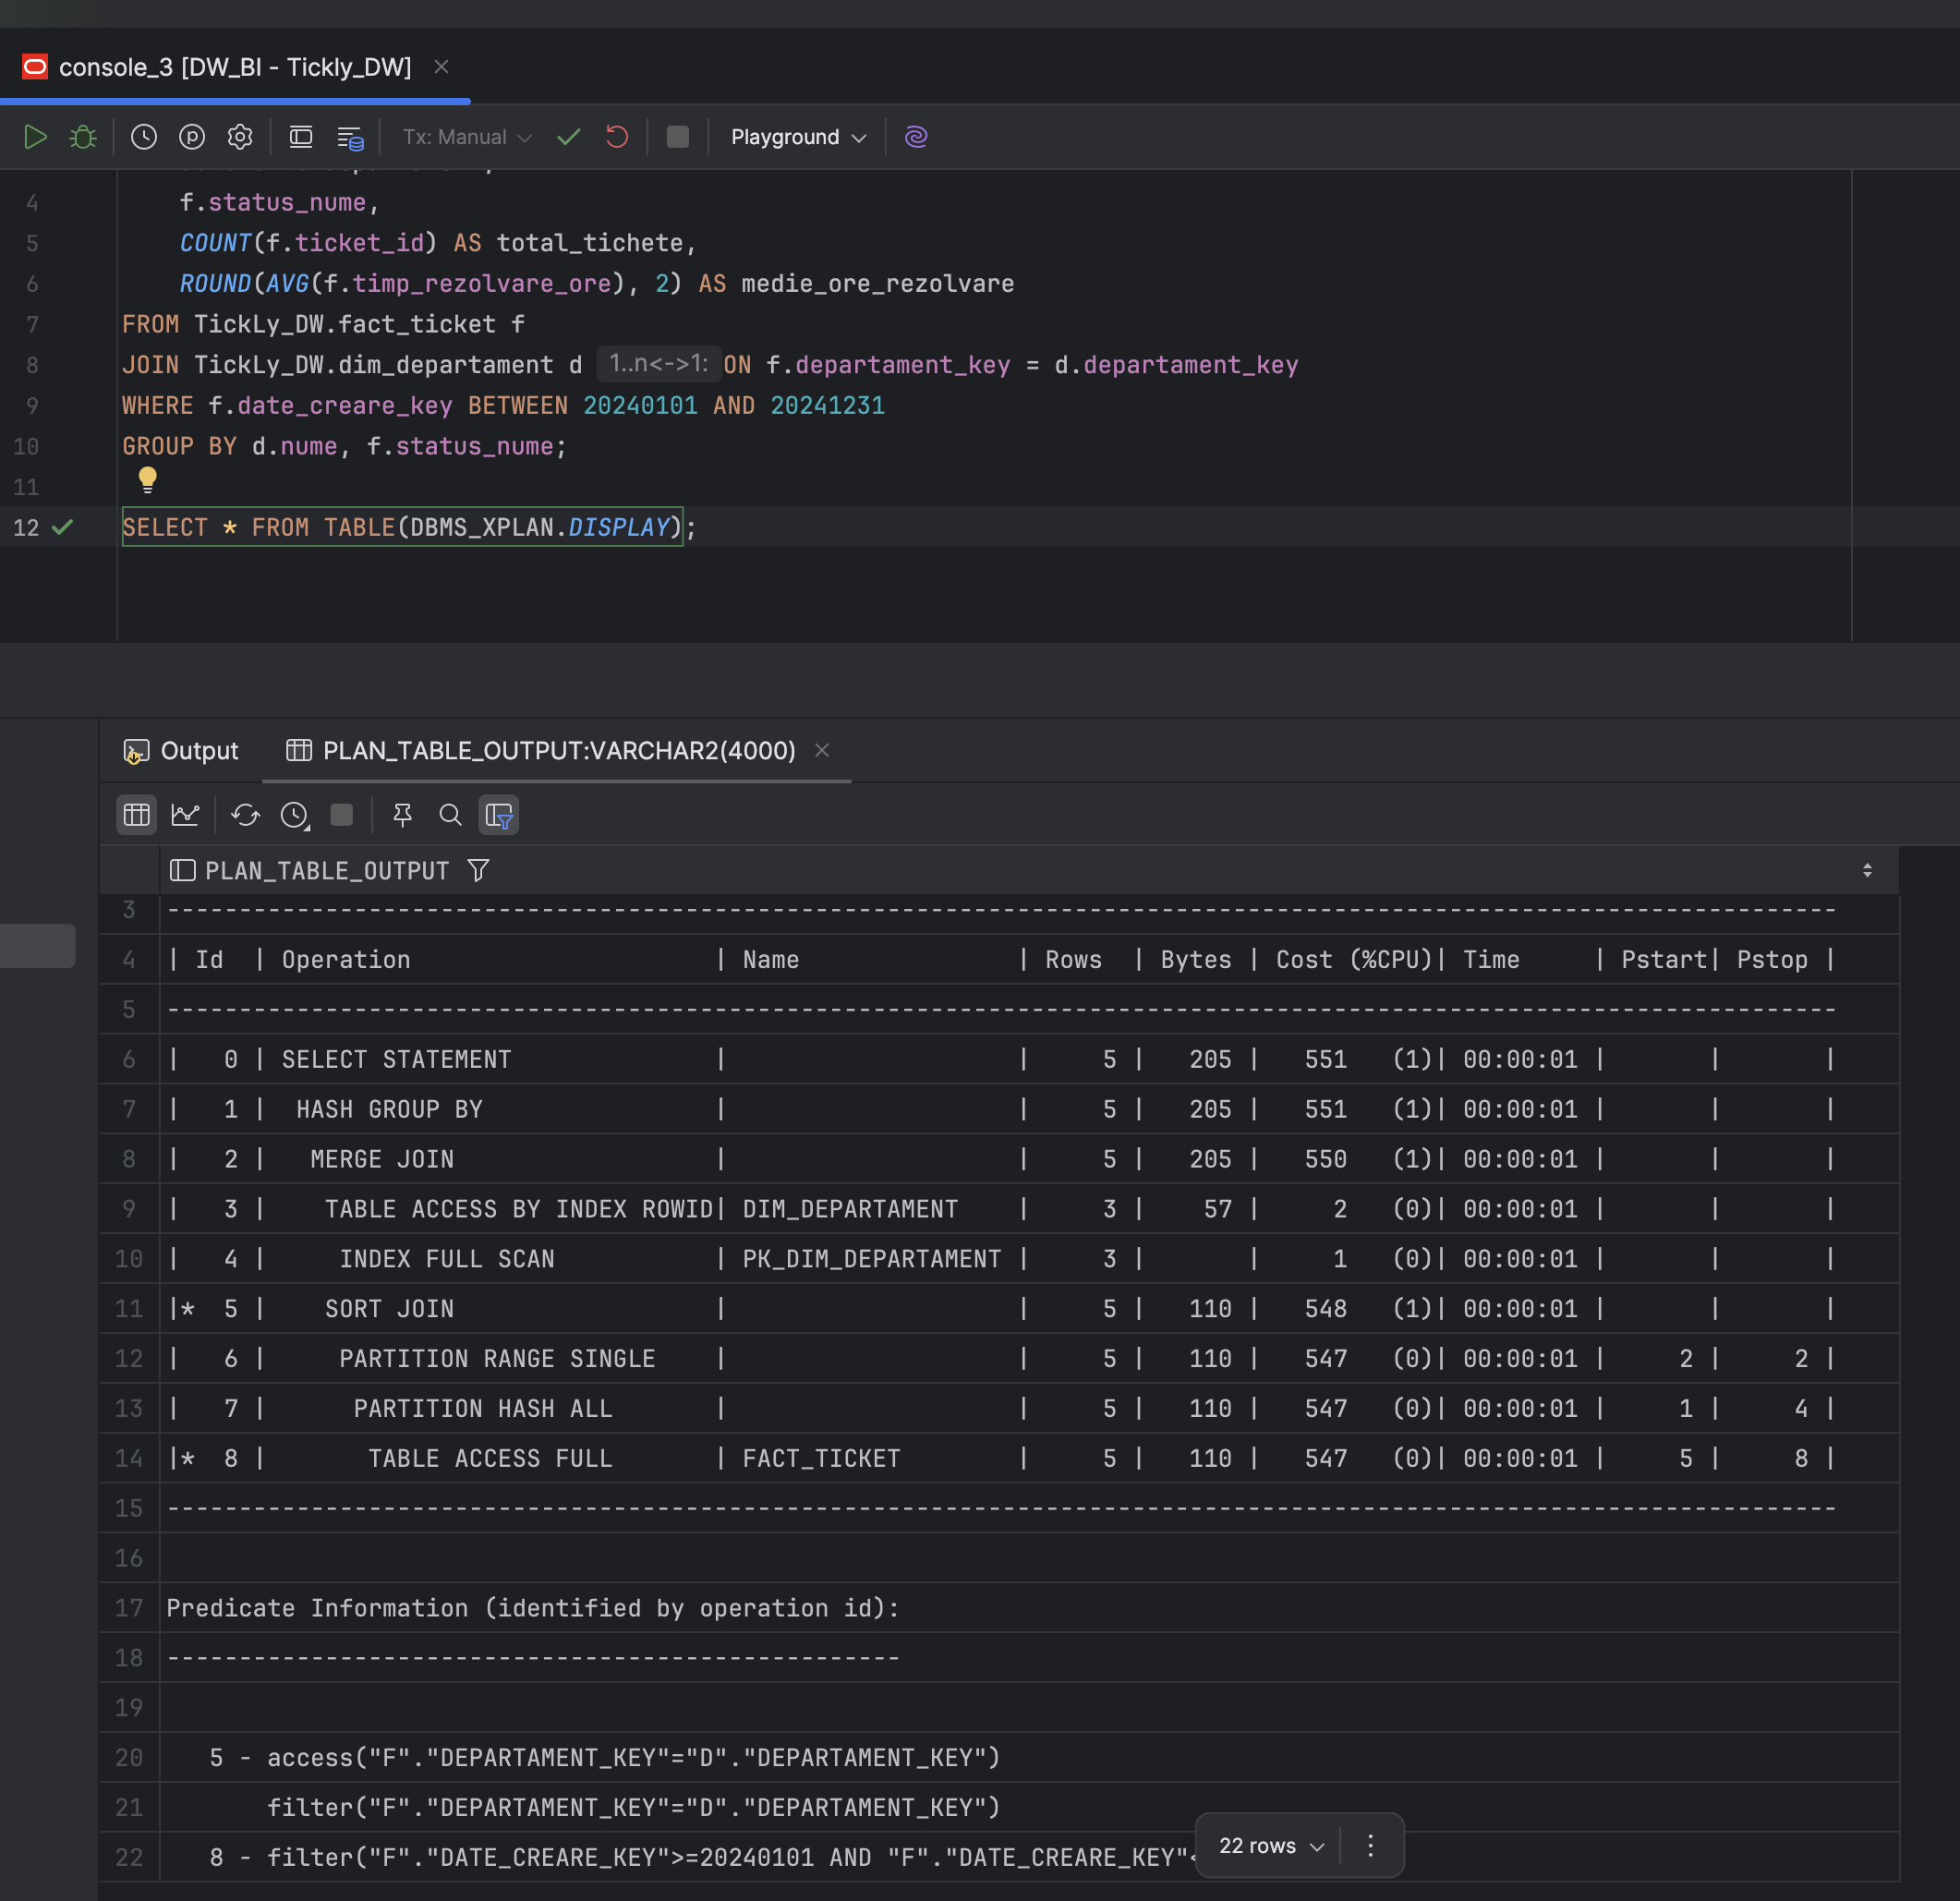
\includegraphics[width=0.6\textwidth]{../../scripts/tests/assets/partitie_range.png}
    \caption{Plan execuție: Partiționare RANGE (PARTITION RANGE SINGLE)}
    \label{fig:partitie_range}
\end{figure}

\textbf{2:} „Analiza performanței pentru un anumit Topic critic (ex: ID 105) în anul 2024.”

\begin{verbatim}
    EXPLAIN PLAN FOR
    SELECT *
    FROM TickLy_DW.fact_ticket f
    WHERE f.date_creare_key BETWEEN 20240101 AND 20241231
      AND f.topic_key = 105;
    
    SELECT * FROM TABLE(DBMS_XPLAN.DISPLAY);
\end{verbatim}

\begin{figure}[H]
    \centering
    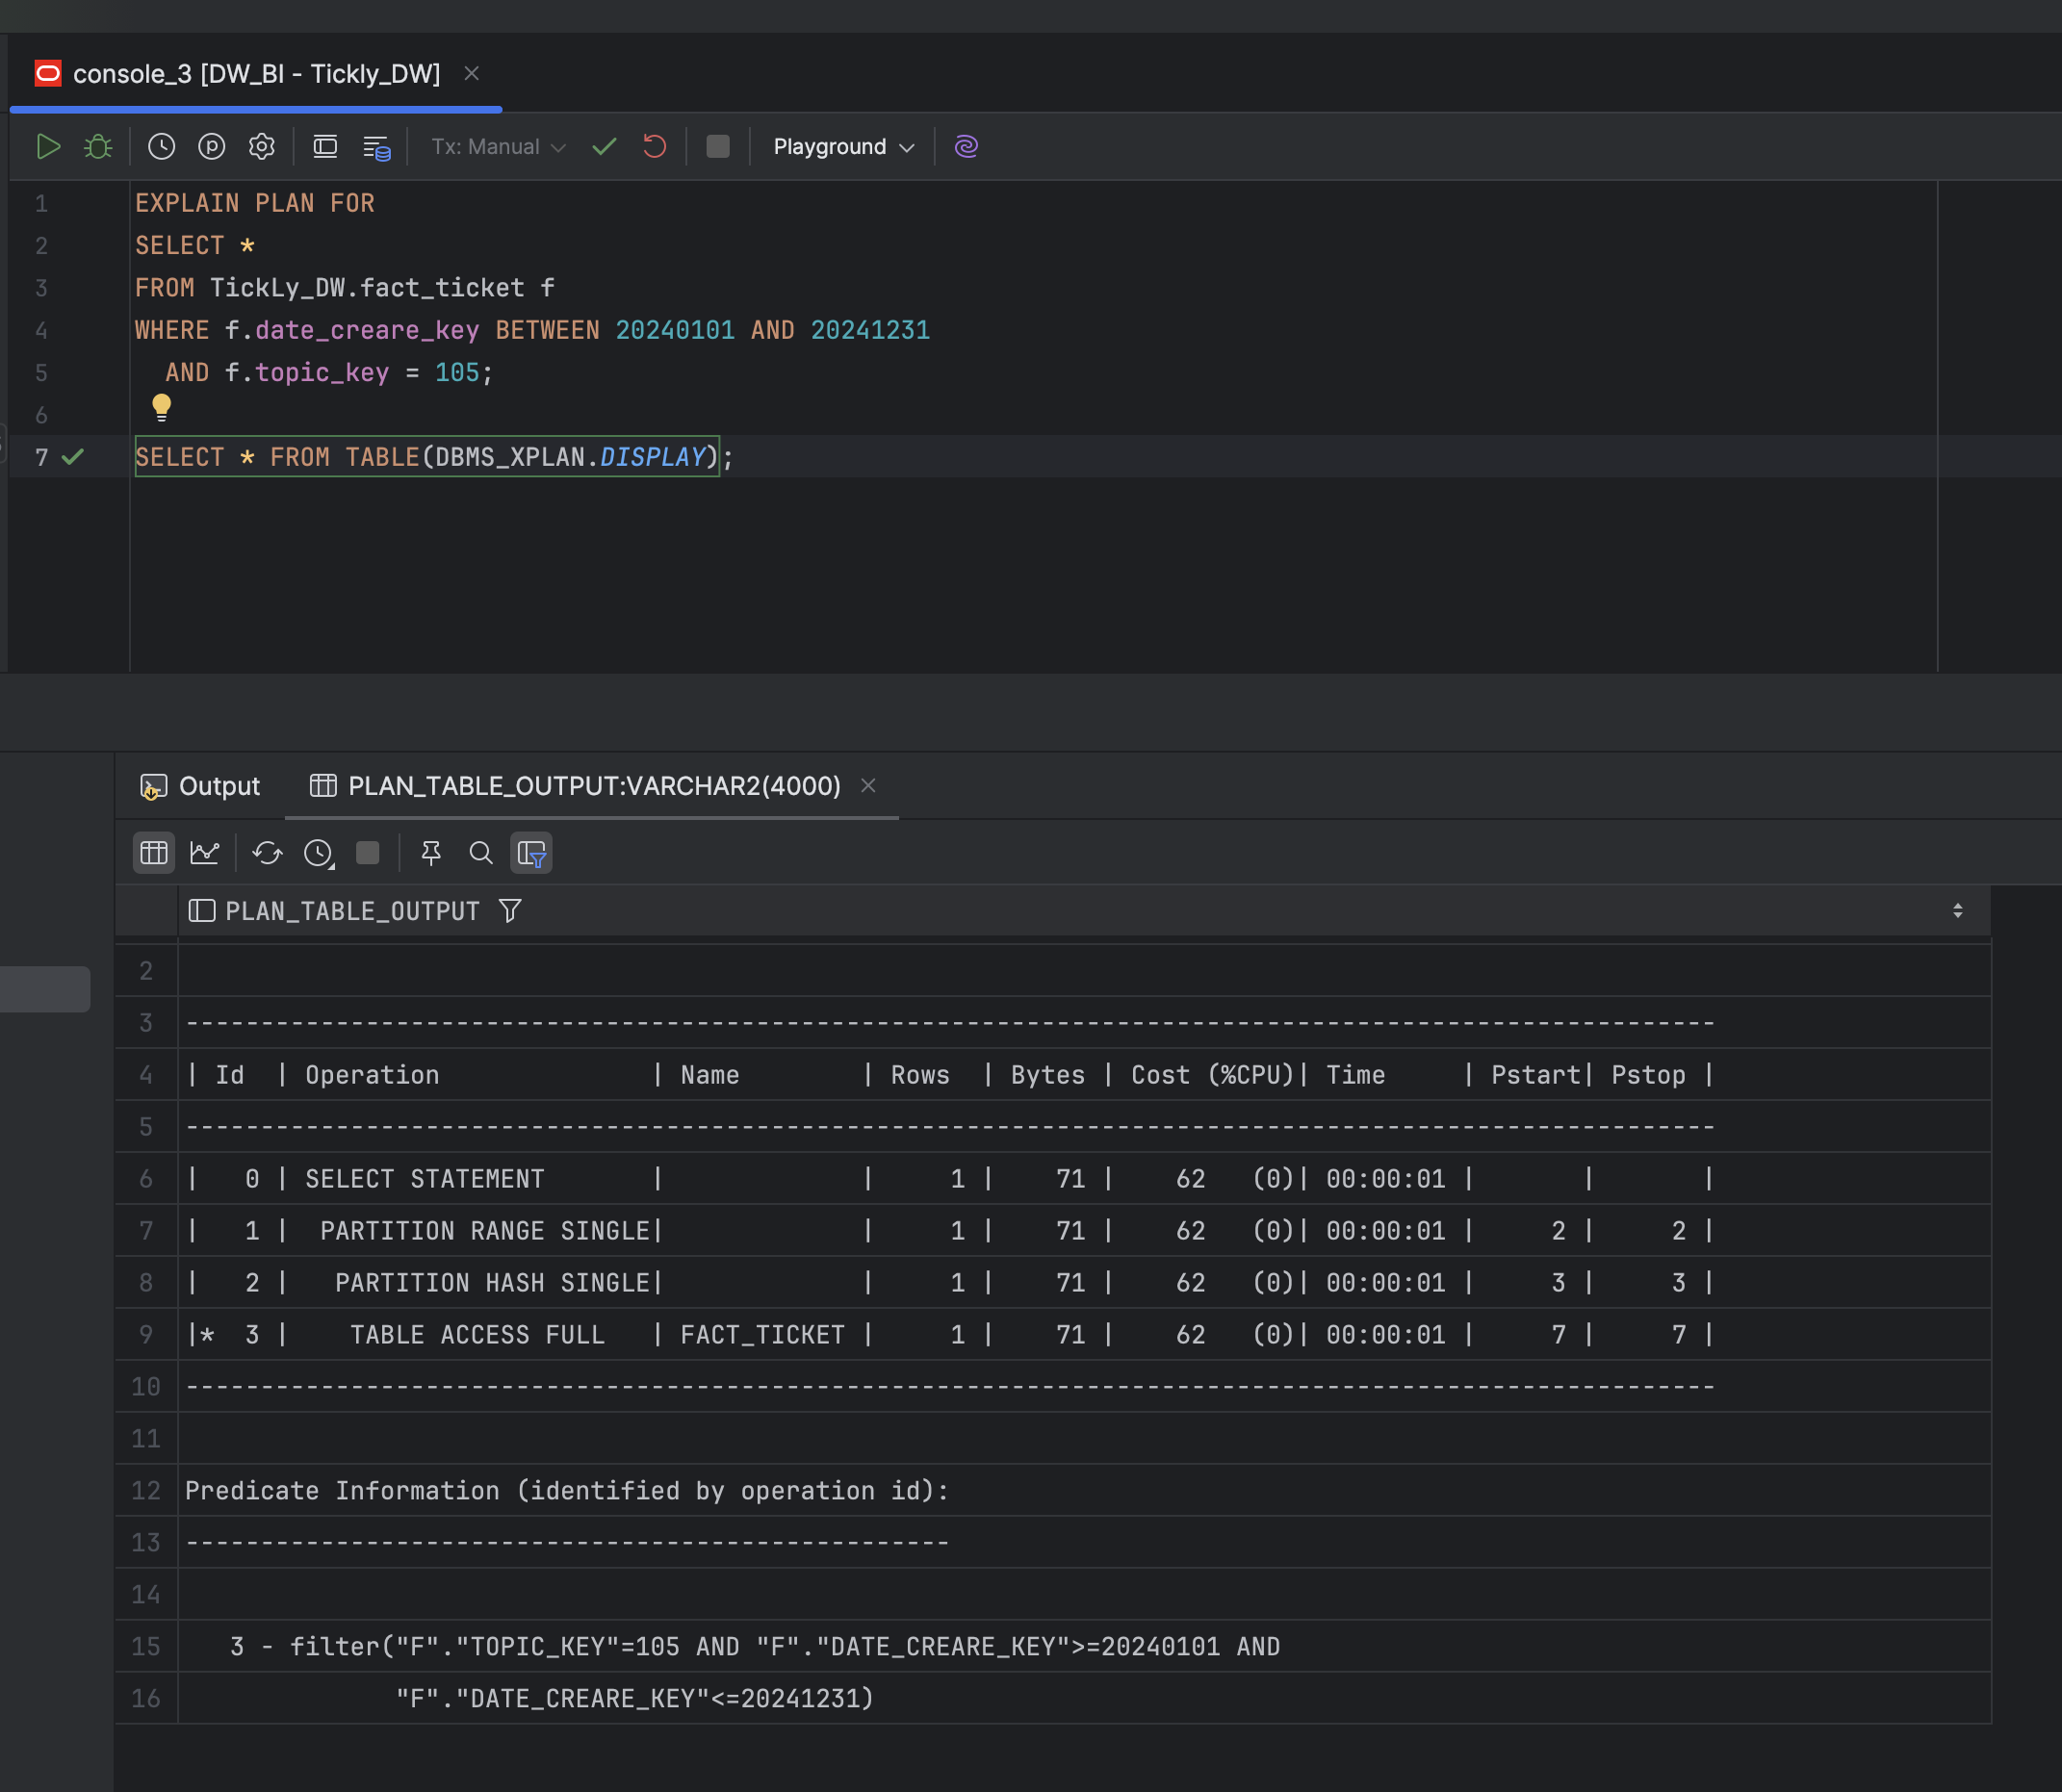
\includegraphics[width=0.6\textwidth]{../../scripts/tests/assets/partitie_range_hash.png}
    \caption{Plan execuție: Partiționare RANGE și HASH}
    \label{fig:partitie_range_hash}
\end{figure}

\textbf{3:} „Lista tuturor clienților persoane juridice și CUI-ul acestora.”

\begin{figure}[H]
    \centering
    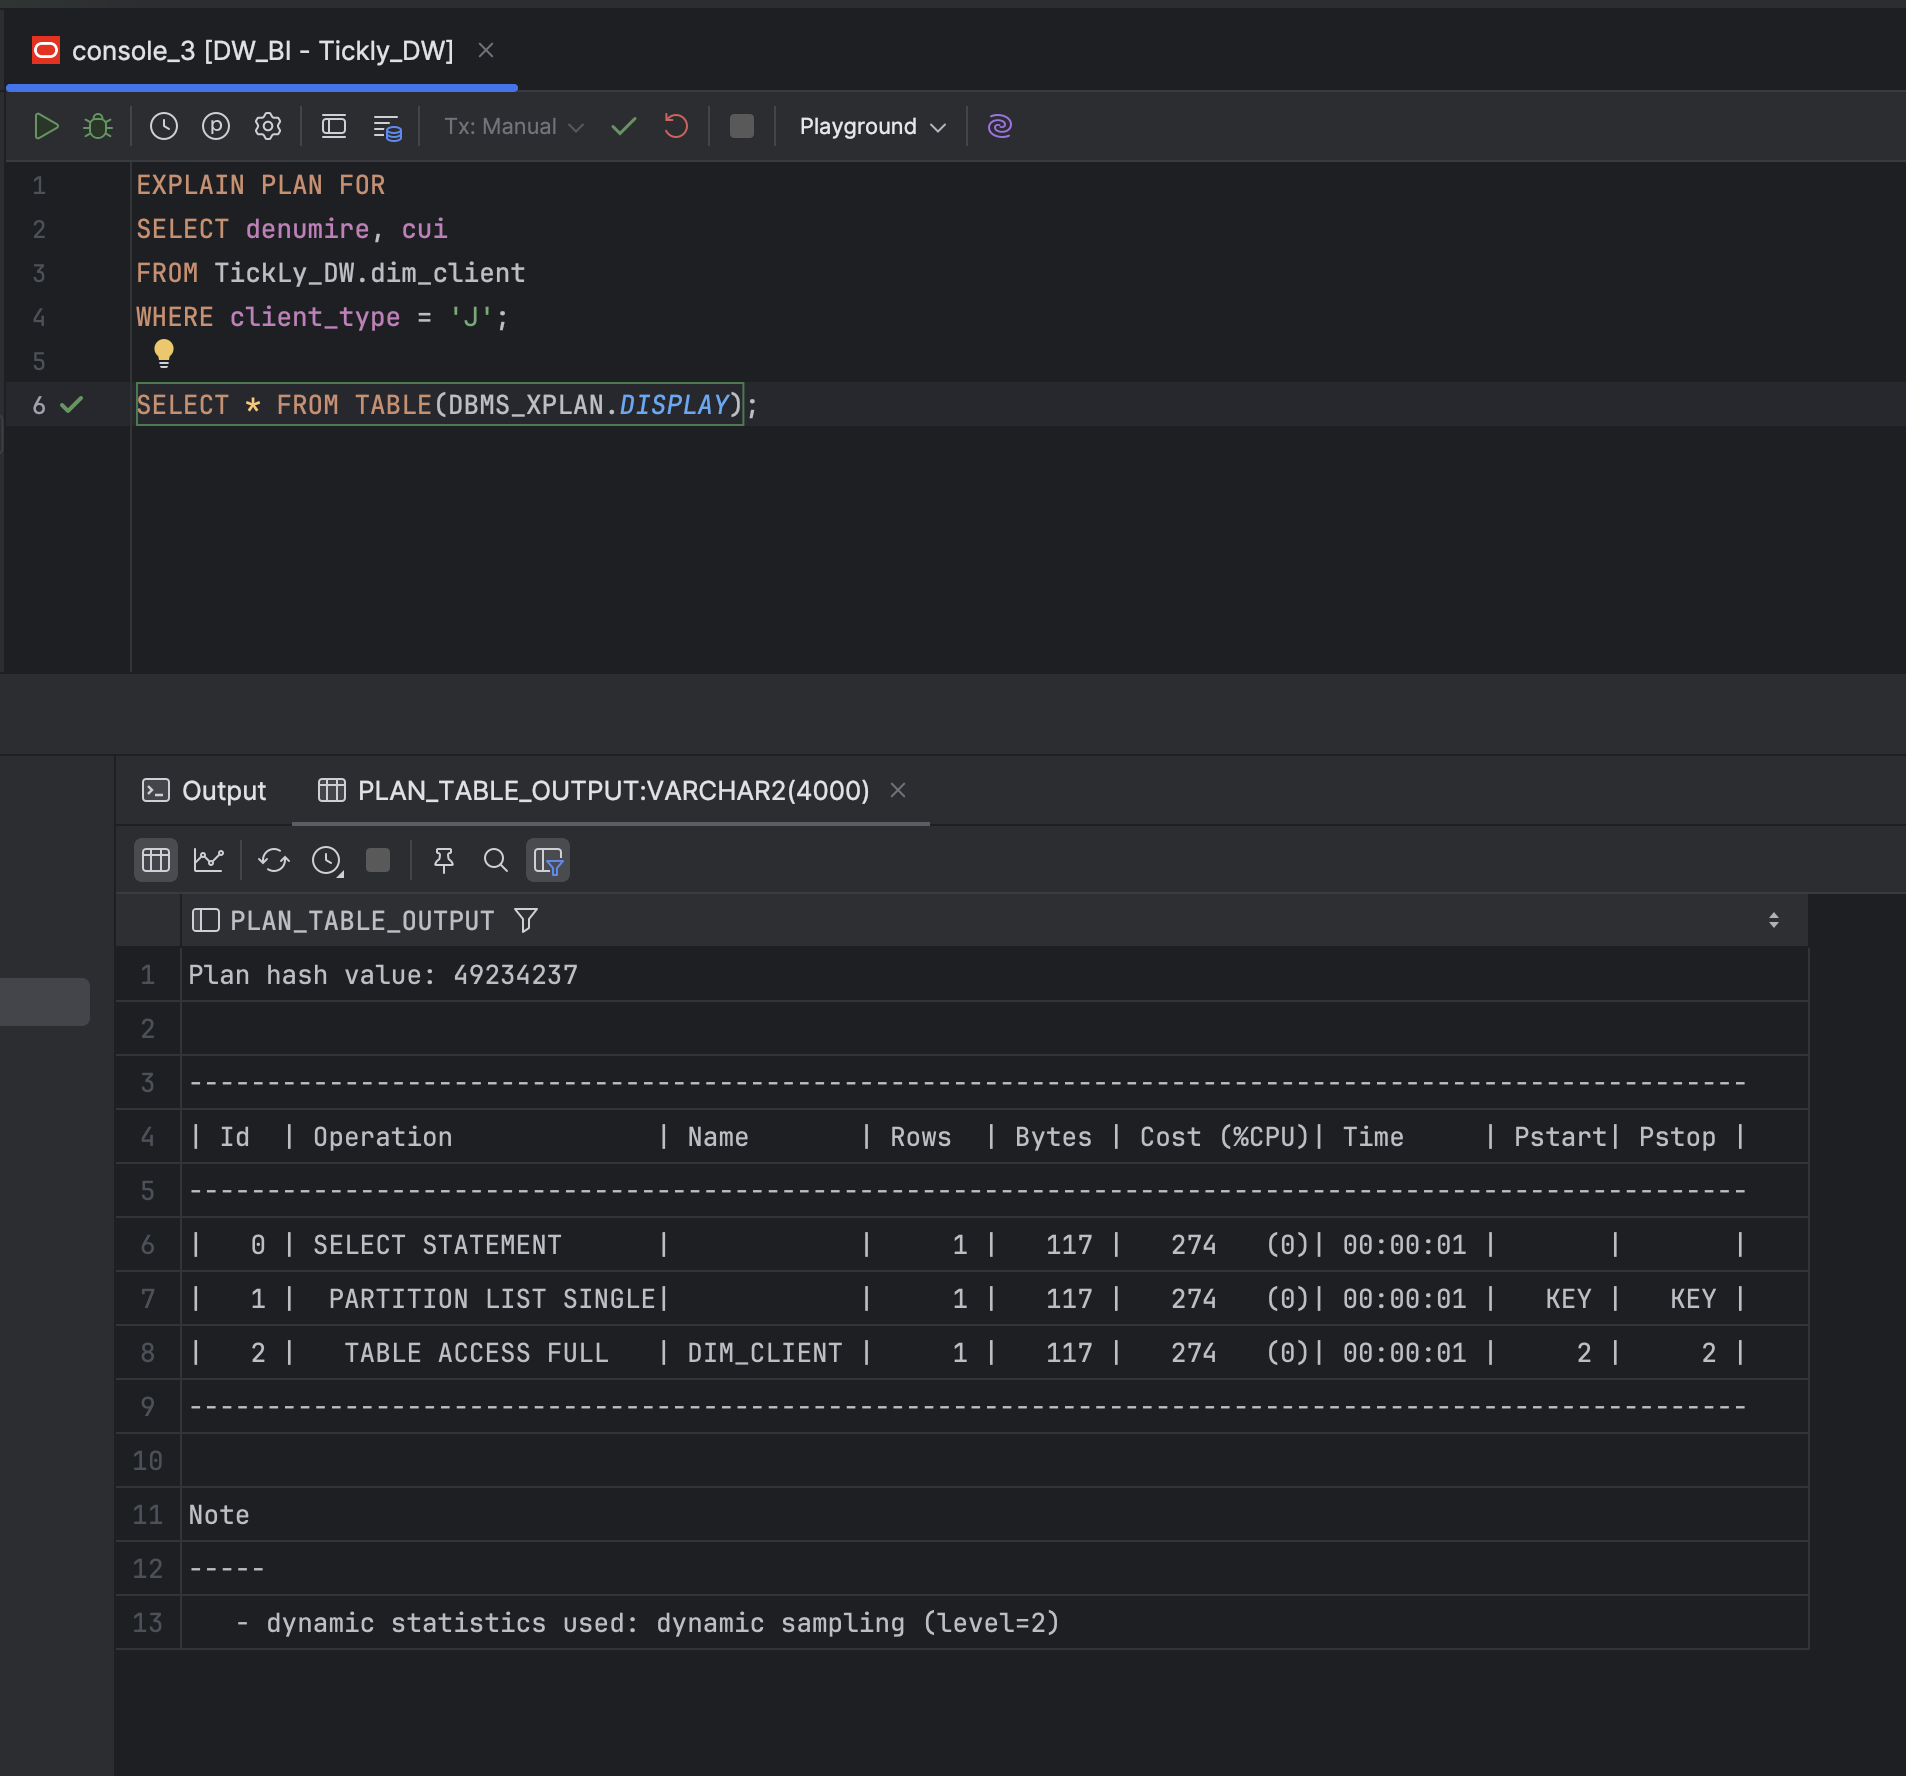
\includegraphics[width=0.6\textwidth]{../../scripts/tests/assets/partitie_list.png} 
    \caption{Plan execuție: Partiționare LIST pe DIM\_CLIENT}
    \label{fig:partitie_list_client}
\end{figure}
